\documentclass[a4paper,14pt]{extarticle}                     % тип документа с размером шрифта 14pt

%---------------------------------------------------------------------------------------------------

%\usepackage{times}                                          % использование Times New Roman
                                                             %     (почему-то сносит все форматирование)
\usepackage[top=2cm,left=3cm,right=1cm,bottom=2cm]{geometry} % размеры полей
\usepackage[]{inputenc}                                      % эта строка нужна, чтобы документ открывался в редакторе MikTex
\usepackage[T2A]{fontenc}                                    % для поддержки русского языка
\usepackage[russian]{babel}                                  % включение русского языка
\usepackage{amsmath,amsthm,amscd,amsfonts,amssymb}           % специальные символы и т.п.
\usepackage{mathrsfs}                                        % специальные символы
\usepackage{indentfirst}                                     % отступ для начала абзаца
\usepackage{textcomp}                                        % текст в формулах
\usepackage{graphicx}                                        % подключение графики
\usepackage{listings}                                        % печать листингов
\usepackage{xcolor}                                          % использование цветов
\usepackage{caption2}                                        % для изменения стиля подписи рисунков
                                                             %     (приводит к warning-у, так что использовать только по необходимости)
\usepackage{verbatim}                                        % использование дополнительных возможностей verbatim           
\usepackage{fancybox}                                        % использование расширенного Verbatim
\usepackage[linesnumbered,boxed]{algorithm2e}                % оформление алгоритмов
\usepackage{booktabs}                                        % поддержка таблиц
\usepackage{makecell}                                        % для перевода строки внутри ячейки таблицы
\usepackage{ulem}                                            % волнистая черта снизу
\usepackage{textcomp}                                        % для коррекции положения тильды
\usepackage{longtable}                                       % многострочные таблицы
\usepackage{morefloats}                                      % подключить большее количество формул
\usepackage[section]{placeins}                               % сброс обработки флотов в конце страницы
\usepackage{float}                                           % расположение флотов прямо тут
\usepackage{setspace}                                        % чтобы менять междустрочный интервал с подписях
\usepackage{cite}                                            % для использования диапазона цитирования

%---------------------------------------------------------------------------------------------------

\lstset{
aboveskip=15pt,
belowskip=15pt,
belowcaptionskip=10pt,
language={[ANSI]C++},
basewidth=0.5em,
xleftmargin=20pt,
xrightmargin=20pt,
basicstyle=\linespread{0.8}\small\ttfamily,                  % 0.8 - уменьшение расстояния между строк
                                                             % linespread должен идти первым 
keywordstyle=\color[rgb]{0,0,1},
numbers=left,
numberstyle=\tiny,
stepnumber=1,
numbersep=10pt,
showspaces=false,
showstringspaces=false,
showtabs=false,
frame=trBL,
tabsize=2,
captionpos=t,
breaklines=false,
breakatwhitespace=false,
escapeinside={\%*}{*)}
}

%---------------------------------------------------------------------------------------------------

%\renewcommand{\GenericWarning}[2]{\GenericError{#1}{#2}{}{This warning has been turned into a fatal error.}} % Предупреждения -> ошибки.
\newcommand{\textapprox}{\raisebox{0.5ex}{\texttildelow}}    % положение тильды
\renewcommand{\baselinestretch}{1.5}                         % полуторный отступ между строк
\renewcommand{\captionlabeldelim}{.}                         % разделитель между номером рисунка и названием
\numberwithin{equation}{section}                             % нумерация формул по секциям
\numberwithin{figure}{section}                               % нумерация картинок по секциям
\numberwithin{table}{section}                                % нумерация таблиц по секциям
\theoremstyle{plain}                                         % стиль теорем
\newtheorem{theorem}{Теорема}[section]                       % теорема
\newtheorem{lemma}{Лемма}[section]                           % лемма
\newtheorem{definition}{Определение}[section]                % определение
\numberwithin{theorem}{section}                              % нумерация теорем по секциям
\numberwithin{lemma}{section}                                % нумерация лемм по секциям
\numberwithin{definition}{section}                           % нумерация определений по секциям

%---------------------------------------------------------------------------------------------------

\captionstyle{center}
\setlength{\abovecaptionskip}{0pt}
\setlength{\belowcaptionskip}{0pt}

%---------------------------------------------------------------------------------------------------

\begin{document}

\numberwithin{lstlisting}{section}                           % нумерация листингов по секциям
                                                             % определяем тут, так как счетчик листинга до begin{document}
                                                             % еще не существует
                                                             % https://tex.stackexchange.com/questions/441618/how-to-number-the-listings-within-sections

\title{Повышение эффективности высокопроизводительных вычислений на поверхностных расчетных сетках с изменяемой геометрией}
\author{Рыбаков~А.~А.}
\date{27.08.2025}
\maketitle
\thispagestyle{empty}                                        % не нумеруем первую страницу

\newpage
\renewcommand{\contentsname}{Оглавление}                     % переопределяем команду перед генерацией оглавления
\tableofcontents

%---------------------------------------------------------------------------------------------------

%\input text_intro.tex                                        % введение
%\input text_2dr.tex                                          % перестроение в двумерном случае
%\input text_3dr.tex                                          % перестроение в трехмерной случае
\input text_int.tex                                          % пересечение с сетками

%---------------------------------------------------------------------------------------------------

%\newpage
%\section*{Глава 2. Методы распаралеливания вычислений с передачей сообщений}                      % выключить номер первой главы
%\addcontentsline{toc}{section}{Глава 2. Методы распаралеливания вычислений с передачей сообщений} % но добавить ее в оглавление
%\addtocounter{section}{1}                                                                                                % а теперь и счетчик продвинуть
%\setcounter{subsection}{0}
%\setcounter{figure}{0}
%\setcounter{equation}{0}
%\setcounter{table}{0}
%\setcounter{theorem}{0}
%\setcounter{lemma}{0}
%\setcounter{definition}{0}
%\setcounter{lstlisting}{0}

%\input text_2_1_qual.tex
%\input text_2_2_block.tex
%\input text_2_3_getero.tex
%\input text_2_4_withcut.tex
%\input text_2_5_decompsurf.tex
%\input text_2_6_smooth.tex
%\input text_2_7_genetic.tex
%\input text_2_8_scaling.tex

%\subsection{Выводы из главы}

%TODO

%---------------------------------------------------------------------------------------------------

%\newpage
%\section*{Глава 3. Методы распараллеливания \\ вычислений на общей памяти}                      % выключить номер первой главы
%\addcontentsline{toc}{section}{Глава 3. Методы распараллеливания вычислений на общей памяти} % но добавить ее в оглавление
%\addtocounter{section}{1}                                                                    % а теперь и счетчик продвинуть
%\setcounter{subsection}{0}
%\setcounter{figure}{0}
%\setcounter{equation}{0}
%\setcounter{table}{0}
%\setcounter{theorem}{0}
%\setcounter{lemma}{0}
%\setcounter{definition}{0}
%\setcounter{lstlisting}{0}

%\input text_3_graph_prim.tex
%\input text_3_edge_coloring.tex
%\input text_3_omp1.tex
%\input text_3_omp2.tex

%\subsection{Выводы из главы}

%TODO

%---------------------------------------------------------------------------------------------------

%\newpage
%\section*{Глава 4. Методы векторизации программного \\ кода для повышения его производительности}                      % выключить номер первой главы
%\addcontentsline{toc}{section}{Глава 4. Методы векторизации программного кода для повышения его производительности} % но добавить ее в оглавление
%\addtocounter{section}{1}                                                                                           % а теперь и счетчик продвинуть
%\setcounter{subsection}{0}
%setcounter{figure}{0}
%\setcounter{equation}{0}
%\setcounter{table}{0}
%\setcounter{theorem}{0}
%\setcounter{lemma}{0}
%\setcounter{definition}{0}
%\setcounter{lstlisting}{0}

%\input text_4_01_vec_description.tex
%\input text_4_02_small_matr.tex
%\input text_4_03_spec_matr.tex
%\input text_4_04_flat.tex
%\input text_4_05_ibm.tex
%\input text_4_06_vec_loc_branch.tex
%\input text_4_07_vec_mrg_under_cond.tex
%\input text_4_08_vec_check_mask.tex
%\input text_4_09_vec_comb_mask.tex

% Опционально можно добавить, тут страницы на 2-3.
%\input text_4_tozh.tex

%\input text_4_10_mesh_intersect.tex
%\input text_4_11_vec_riemann.tex
%\input text_4_12_vec_irreg.tex
%\input text_4_13_vec_integer.tex

%\subsection{Выводы из главы}

%\begin{figure}[ht]
%\centering
%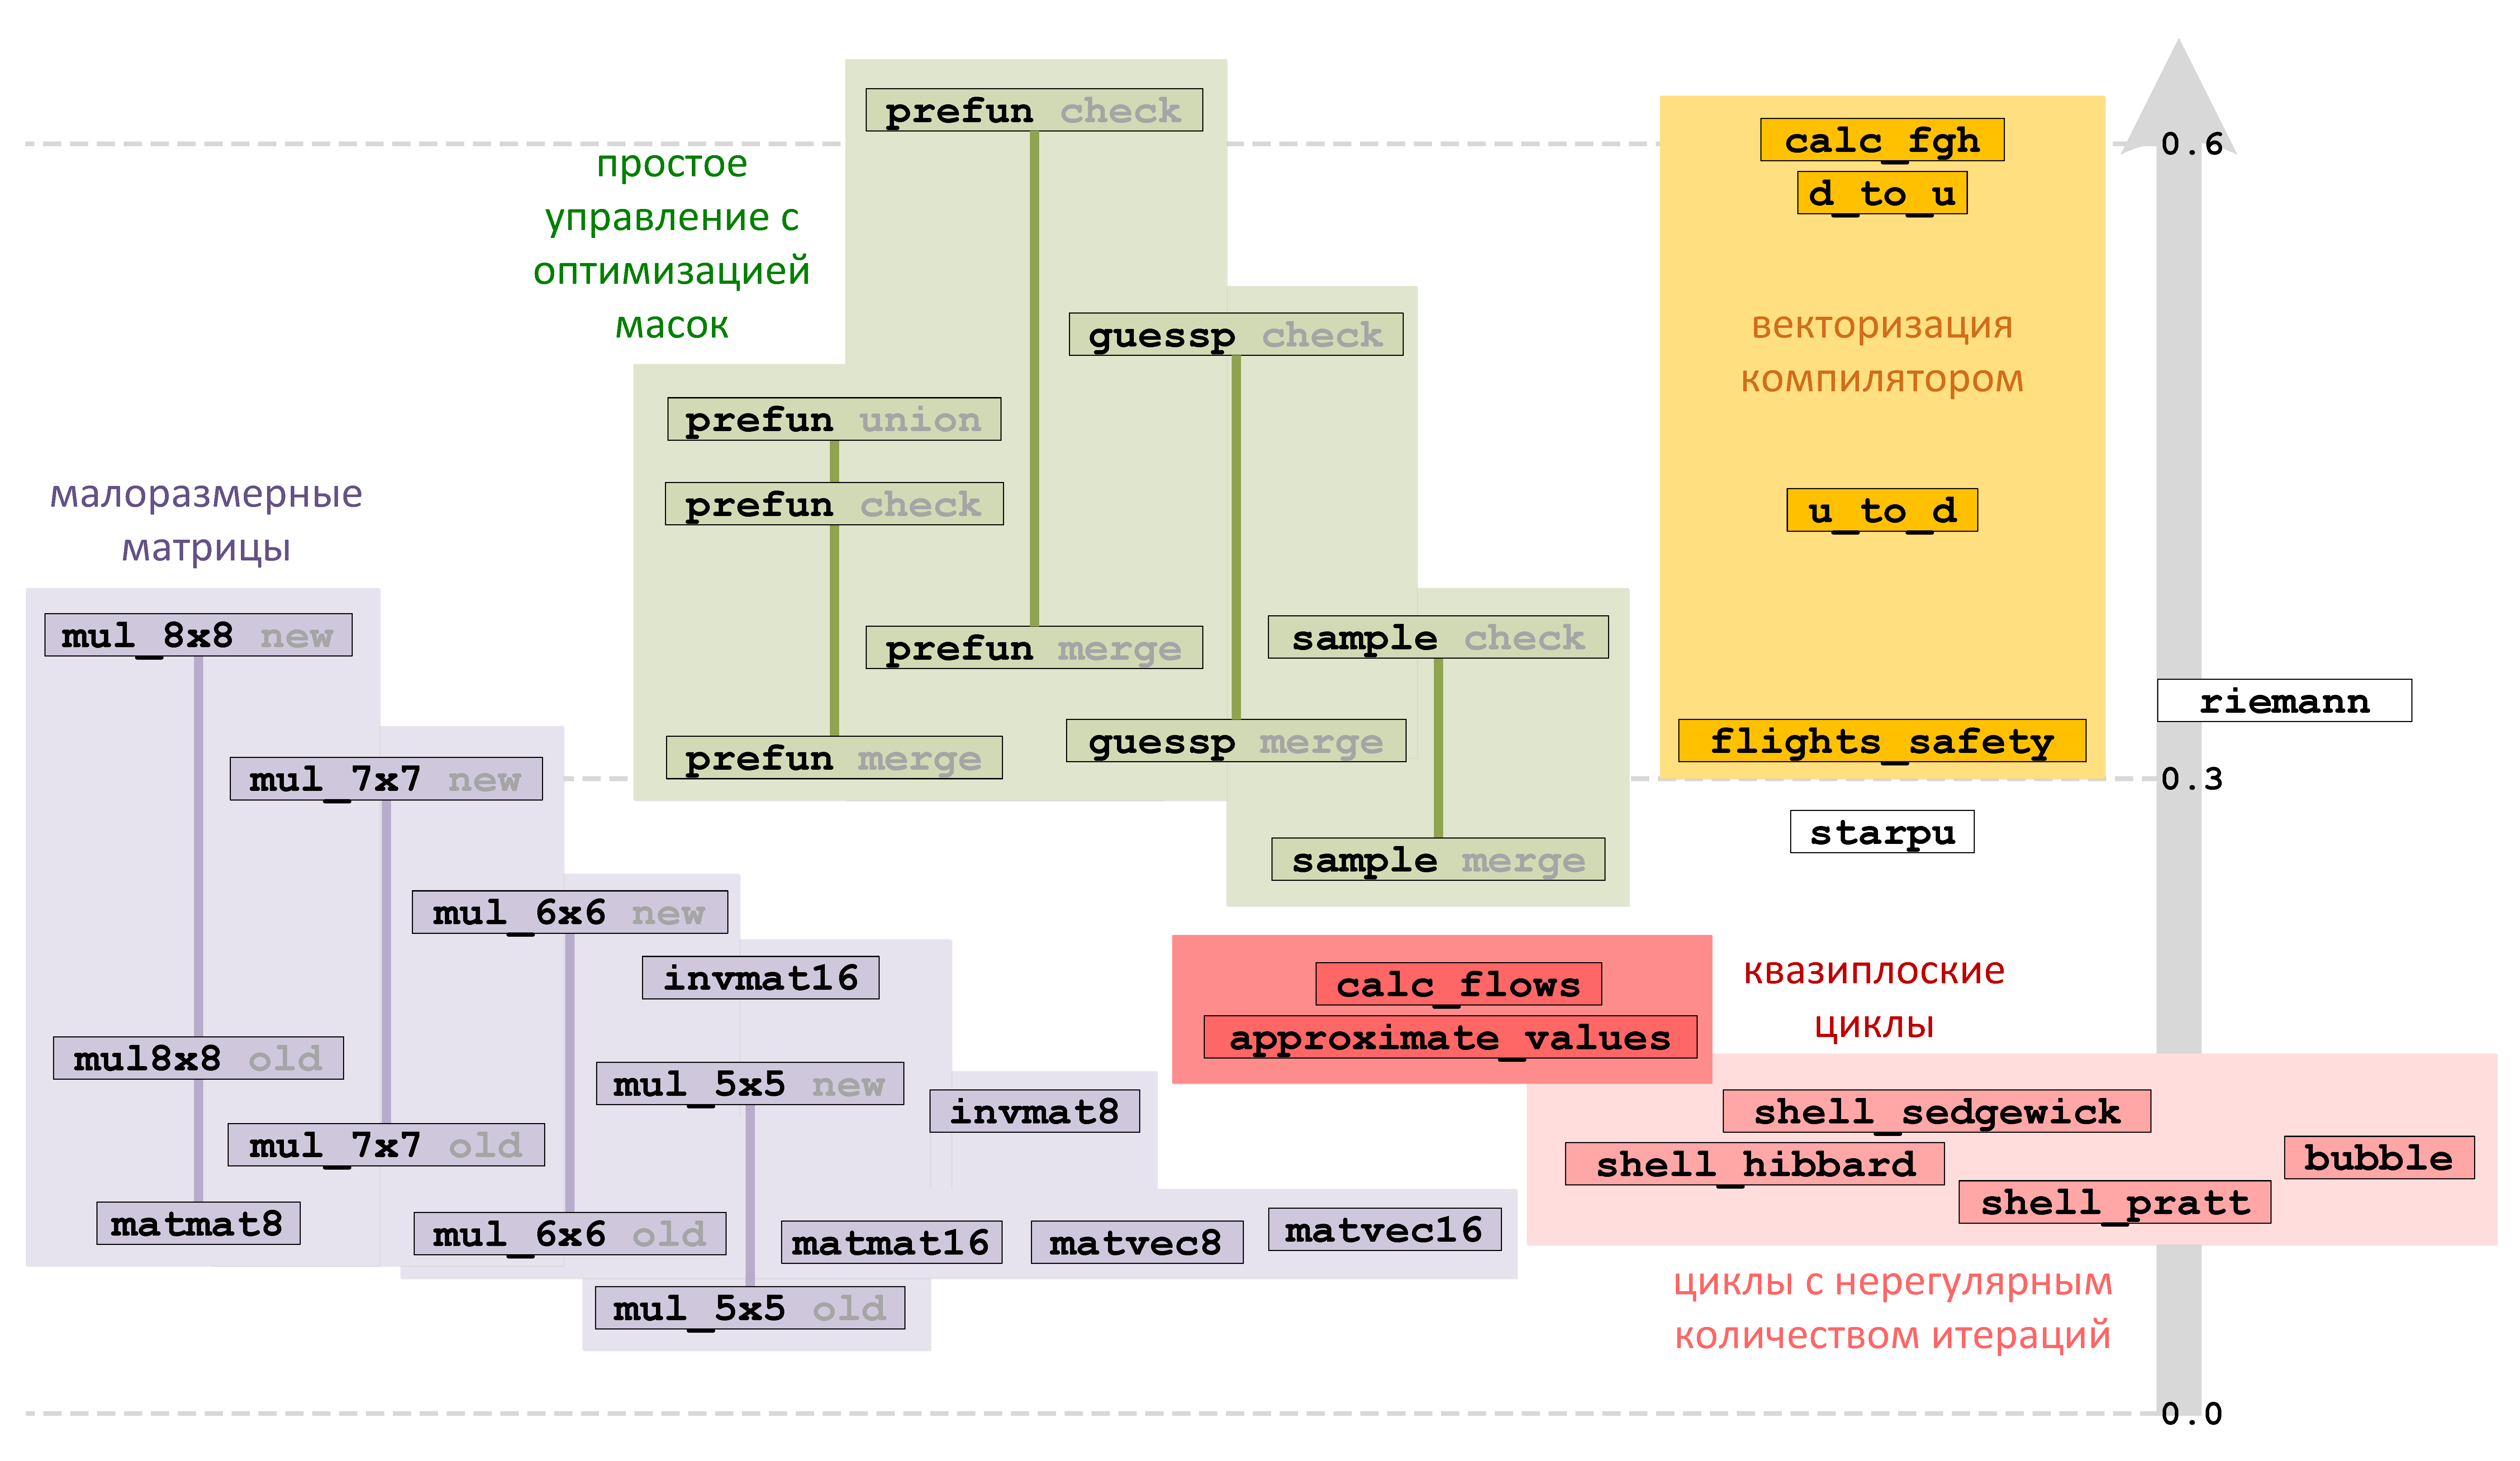
\includegraphics[width=1.0\textwidth]{./pics/text_4_fin/map_cut.pdf}
%\singlespacing
%\captionstyle{center}\caption{Карта эффективности векторизации.}
%\label{fig:text_4_fin_map}
%\end{figure}

%Векторизация\label{term:vectorization7} является важной низкоуровневой оптимизацией программного кода, с помощью которой можно достичь кратного ускорения суперкомпьютерных приложений.
%Все основные современные микропроцессорные архитектуры поддерживают векторные вычисления, причем наблюдается тенденция на увеличение размера вектора (на сегодняшний день максимальная длина равна 512 битам, но уже сейчас логически эта длина не ограничена, учитывая наборы векторных инструкций с переменной длиной вектора).

%Сейчас наиболее перспективным набором векторных инструкций является набор AVX-512\label{abbr:avx9}, так как в нем поддержана возможность выборочной обработки элементов векторов с помощью векторных масок\label{term:vector_mask9}.
%Эта уникальная возможность позволяет векторизовать сложный программный контекст, содержащий команды передачи управления, гнезда циклов и вызовы функций.

%В этой главе были рассмотрены и предложены новые методы векторизации программного кода.
%На рис.~\ref{fig:text_4_fin_map} приведена карта сравнения программного контекста различного вида по эффективности векторизации $e_{vec}$.
%На этом рисунке схожие по свойствам тестовые примеры объединены в одной цветовой гамме.
%Многие из представленных тестовых примеров векторизации программного кода были использованы при численном решении задач обледенения и газовой динамики.

%В разделах \ref{sec:text_4_small_matr}, и \ref{sec:text_4_spec_matr} продемонстрированы подходы к векторизации матричных операций малой размерности.
%При выполнении векторизации программного кода необходимо уметь находить наборы однотипных операций для объединения их в векторные операции над векторными наборами данных.
%При этом полнота использования элементов векторных данных в вычислениях, выраженная в высокой плотности векторных масок\label{term:vector_mask_density7}, напрямую влияет на эффективность векторизации\label{term:vec_eff8} (см. риc.~\ref{fig:text_4_fin_map}, малоразмерные матрицы).

%В разделе \ref{sec:text_4_flat} введено понятие плоского цикла\label{term:flat_loop6}, с помощью которого предпринимается попытка унифицировать процесс объединения однотипных операций в векторные инструкции путем записи тела плоского цикла в предикатной форме\label{term:predicate_view5} с последущей векторизацией с помощью замены скалярных операций векторными аналогами.
%Можно констатировать, что плоский цикл может быть векторизован при практически произвольном виде его тела (тело может содержать сложное управления, гнезда циклов, вызовы функций).

%В разделе \ref{sec:text_4_ibm} приведено описание подхода, как вычисления могут быть представлены в виде композиции плоских циклов с относительно простым телом, после чего успешно векторизованы оптимизирующим компилятором в автоматическом режиме (см. рис.~\ref{fig:text_4_fin_map}, \texttt{calc\_fgh}, \texttt{calc\_d\_to\_u}, \texttt{calc\_u\_to\_d}).
%При этом рассматривается предпочтительный способ организации хранения данных в виде <<набора массивов>> и оптимизация расщепления гнезда циклов по условию\label{term:loop_split_by_cond4} для уменьшения количества операций передачи управления внутри плоского цикла.
%Отмечено, что цикл, не являющийся в полной мере плоским (квазиплоский цикл)\label{term:flat_kvazy_flat2}, также может быть успешно векторизован, но с некоторой потерей производительности (см. рис.~\ref{fig:text_4_fin_map}, \texttt{calc\_flows}).

%Так как основной преградой к эффективной векторизации является наличие операций передачи управления внутри тела плоского цикла (операция передачи управления не может быть векторизована), то в разделе \ref{sec:text_4_loc_branch} рассматриваются оптимизации, направленные на избавление от условий внутри цикла.
%Рассматривается оптимизация выноса маловероятного региона из цикла\label{term:meth_vec_del_low_prob_regions3} и поставлен эксперимент по определению эффективности автоматической векторизации при использовании этой оптимизации (см. рис.~\ref{fig:text_4_fin_map}, \texttt{flights\_safety}).
%Приведено описание оптимизации <<черная дыра>>\label{term:blackhome_optimization2} по выделению вероятного пути исполнения в теле плоского цикла.

%В разделе \ref{sec:text_4_vec_mrg_under_cond} приведено описание и теоретическая оценка общего подхода к избавлению от операций передачи управления и слиянию путей исполнения\label{term:meth_vec_merge4} в теле плоского цикла с помощью векторных инструкций blend.

%В разделе \ref{sec:text_4_vec_check_mask} описывается простая операция проверки векторных масок на пустоту\label{term:meth_vec_check4}, которая оказывает наибольший прирост производительности при векторизации простого программного контекста (см. рис.~\ref{fig:text_4_fin_map}, функции с пометкой \texttt{check}).

%В разделе \ref{sec:text_4_comb_mask} предлагается метод объединения векторных масок\label{term:meth_vec_union3}, позволяющих одновременно исполнять блоки векторных инструкций с непересекающимися масками (см. рис.~\ref{fig:text_4_fin_map}, \texttt{prefun union}).
%Также предлагается метод комбинирования векторных масок\label{term:meth_vec_comb2}, позволяющий одновременно исполнять блоки векторных инструкций с пересекающимися масками.

%Остальные разделы посвещены методам векторизации гнезд циклов, в которых один из циклов является плоским.

%Наиболее простым случаем является векторизаци гнезда циклов с постоянным количеством итераций, так как в этом случае условие выхода из цикла не требует векторизации.
%Этот случай рассмотрен в разделе \ref{sec:text_4_vec_mesh_intersect} и продемонстрировал лучшую эффективность среди примеров векторизации гнезд циклов (см. рис~\ref{fig:text_4_fin_map}, \texttt{tri\_box\_intersect}).

%В разделе \ref{sec:text_4_vec_riemann} расмсотрен пример векторизации гнезда циклов с непостоянным количеством итераций для расчетной задачи, в которой условие выхода из цикла на разных итерациях плоского цикла меняется медленно.
%Векторизация такого гнезда циклов возможна с помощью векторизации условия выхода из цикла, и эффективность векторизации оказывается ниже, чем в примере с постоянным количеством итераций (см. рис.~\ref{fig:text_4_fin_map}, \texttt{starpu}).

%Наиболее сложным для векторизации случаем является векторизация гнезд циклов с нерегулярным количеством итераций.
%Такой программый контекст рассмотрен в разделах \ref{sec:text_4_vec_irreg} (вещественные вычисления) и \ref{sec:text_4_integer} (целочисленные вычисления).
%При этом внутри итерации плоского цикла векторизуемые условия оказываются непредсказуемыми, что приводит к понижению плотности векторных масок\label{term:vector_mask_density8} в векторных инструкциях и падению производительности (см. рис.~\ref{fig:text_4_fin_map}, циклы с нерегулярным количеством итераций).
%Такой программный контекст характерен для дискретных задач и он демонстрирует наиболее низкую эффективность векторизации.

%---------------------------------------------------------------------------------------------------

%\newpage
%\section*{Заключение}                                        % выключить номер заключения
%\addcontentsline{toc}{section}{Заключение}                   % но добавить его в оглавление

%---------------------------------------------------------------------------------------------------

\input text_abbr.tex         % список сокращений
\input text_term.tex
\input text_bibliography.tex % список используемой литературы

%---------------------------------------------------------------------------------------------------

\end{document}
